\chapter[Resultados]{Resultados}
\label{cp:resultados}

O Grata foi desenvolvido utilizando o \textit{Python Rest} como \textit{Backend} e o \textit{React} como \textit{Frontend}. Para facilitar futuras evoluções foi utilizado o \textit{Dcoker} e o \textit{Deploy} foi realizado na plataforma \textit{Heroku}. Tudo desenvolvido para este projeto pode ser encontrado nos repositórios:
\begin{itemize}
    \item Documentação Grata: \url{https://github.com/FGAProjects/TCC};
    \item Frontend: \url{https://github.com/FGAProjects/Grata-Frontend};
    \item Backend: \url{https://github.com/FGAProjects/Grata-Backend}.
\end{itemize}

O links dos deploys da ferramenta:
\begin{itemize}
    \item Backend: \url{https://api-grata.herokuapp.com/}
    \item Frontend: \url{https://projeto-grata.herokuapp.com/}
\end{itemize}

\section{Ferramenta}

A seguir algumas imagens da ferramenta desenvolvida:

\begin{figure}[H]
    \centering
    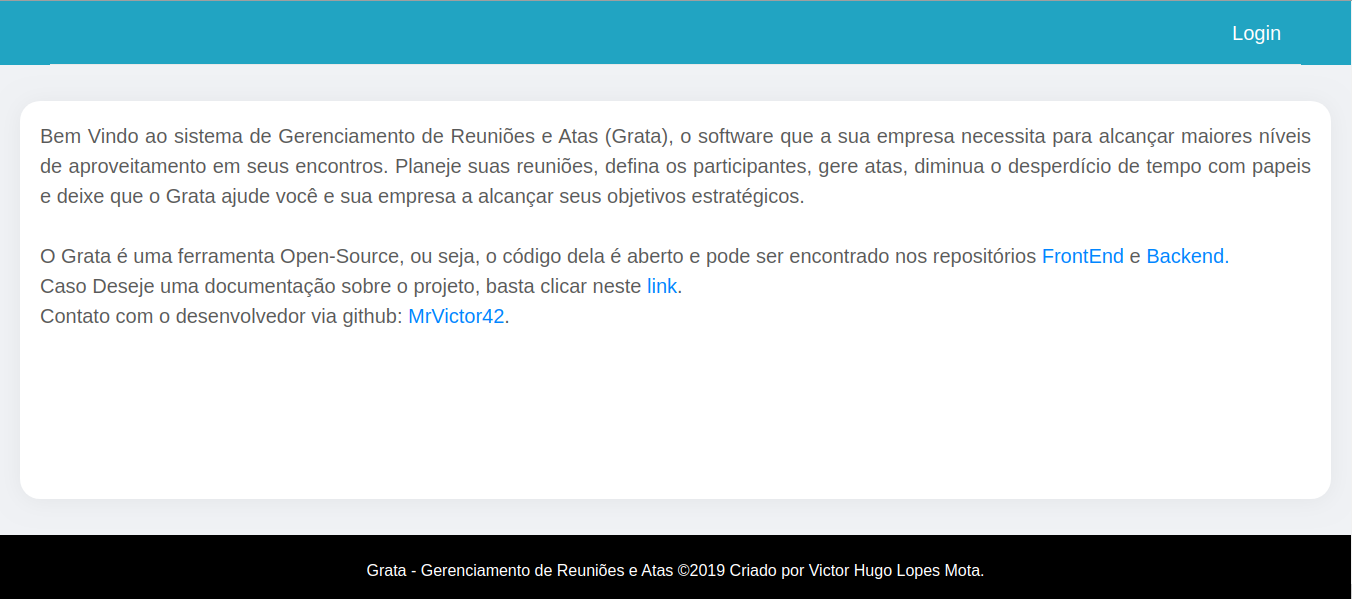
\includegraphics[width=1.0\textwidth]{figuras/grata_login.png}
    \caption{Login Grata. Fonte: Própria}
    \label{img:grata_login}
\end{figure}

\begin{figure}[H]
    \centering
    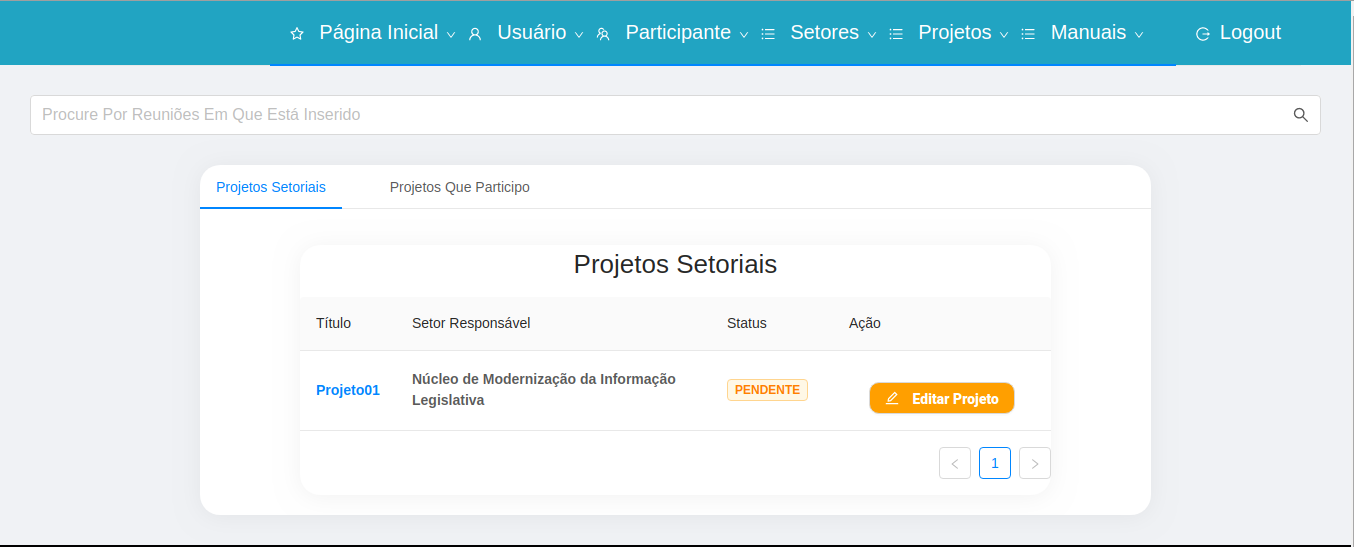
\includegraphics[width=1.0\textwidth]{figuras/pagina_inicial_grata.png}
    \caption{Página Inicial Grata. Fonte: Própria}
    \label{img:pagina_inicial_grata}
\end{figure}

\begin{figure}[H]
    \centering
    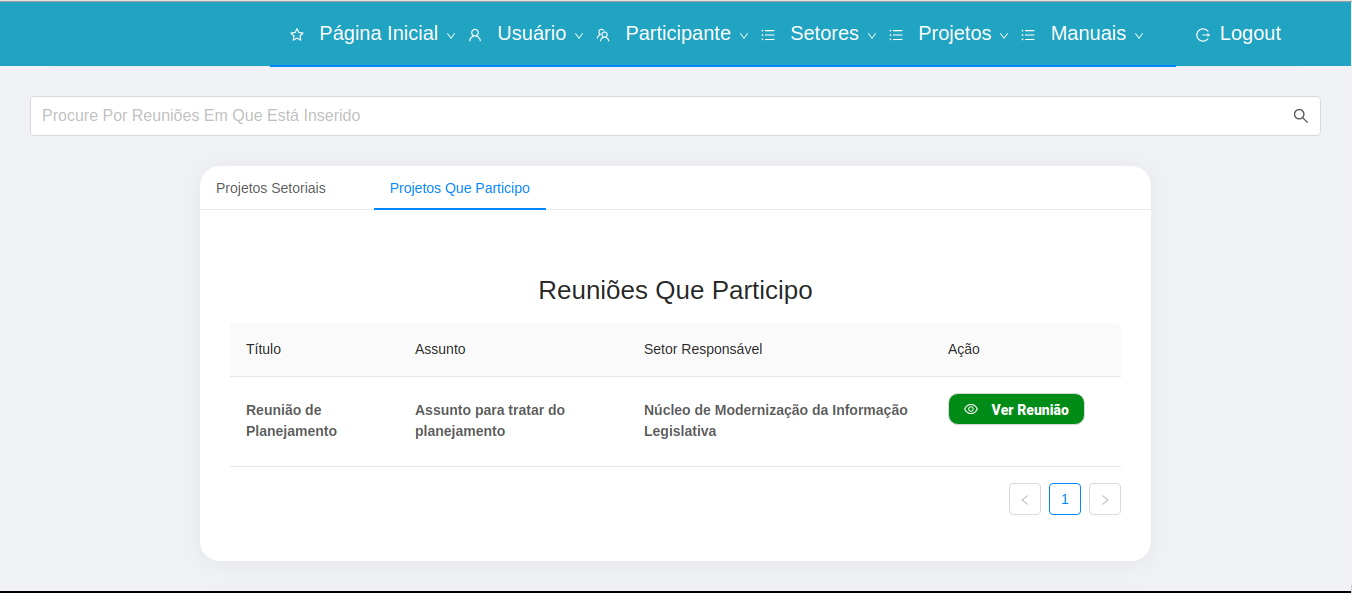
\includegraphics[width=1.0\textwidth]{figuras/reunioes_que_participo.png}
    \caption{Reuniões Que Participo. Fonte: Própria}
    \label{img:reunioes_que_participo}
\end{figure}

\begin{figure}[H]
    \centering
    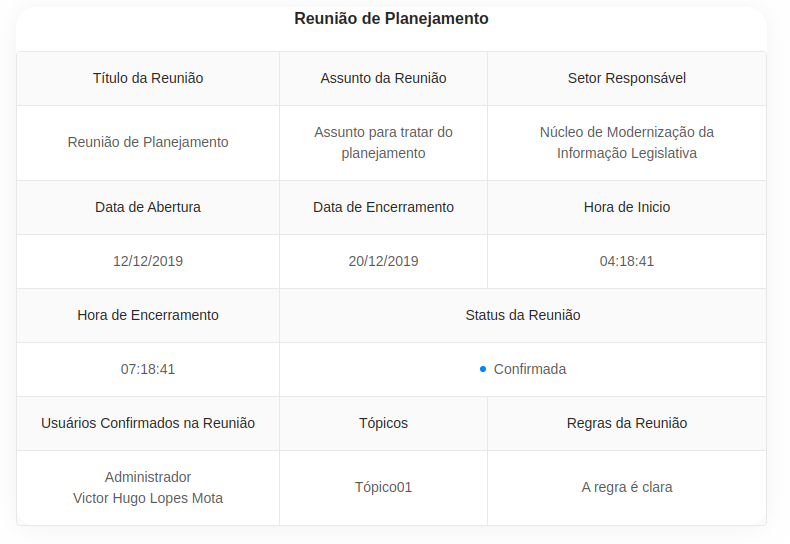
\includegraphics[width=1.0\textwidth]{figuras/ata.png}
    \caption{Ata. Fonte: Própria}
    \label{img:ata}
\end{figure}

\begin{figure}[H]
    \centering
    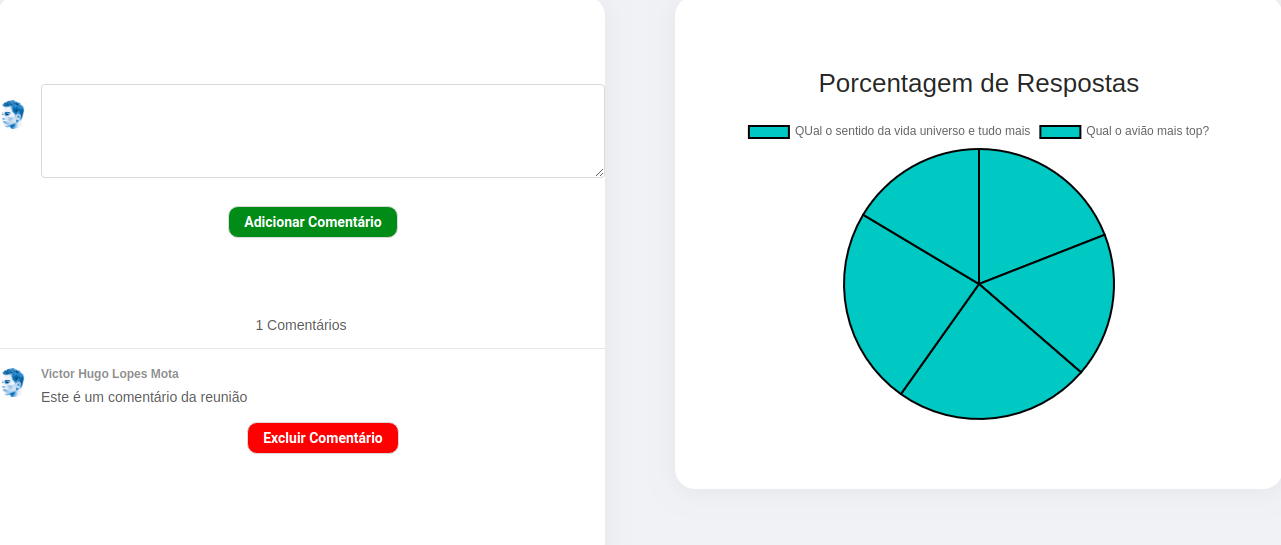
\includegraphics[width=1.0\textwidth]{figuras/resultados_questionario.png}
    \caption{Resultados Questionário. Fonte: Própria}
    \label{img:resultados_questionario}
\end{figure}